\documentclass{article}
%\usepackage[spanish,activeacute]{babel}
%\usepackage[english,activeacute]{babel}
%\usepackage[latin1]{inputenc}
\usepackage[utf8]{inputenc}
\usepackage[english]{babel}

\usepackage{amsmath,amsfonts,amssymb,amstext,amsthm,amscd}
\usepackage{hyperref}
\usepackage{latexsym}
\usepackage{graphicx}
%\usepackage{subfigure}
\usepackage{subfig}
%\linespread{1.6}
\usepackage{float}
\usepackage{dcolumn}% Align table columns on decimal point(esto lo saque del ejemplo de revtex4)
\usepackage{bm}% bold math(esto lo saque del ejemplo de revtex4)
\newcounter{itemR}
\usepackage{here} %recordar usar el comando[H] para las gráficas que es el comando here en lugar de [h!]
\usepackage{fancyhdr}
%\usepackage{sidecap}
%\usepackage[spanish,activeacute]{babel}
\usepackage{multirow}
\usepackage{multicol}
\usepackage{array}
\usepackage{enumitem}
%\usepackage{booktabs}% para hacer tablas profesionales con \toprule

% ------------------------------------------------------------------------------------------------------------------------------------------------------

\usepackage{fancyhdr}
\setlength{\headheight}{15.2pt}
\usepackage[paperwidth=8.5in, paperheight=11.0in, top=1.0in, bottom=1.0in, left=1.0in, right=1.0in]{geometry}

\pagestyle{fancyplain}
\fancyhead[LE,RO]{Práctica $\#$8}
\fancyhead[CE,CO]{}
\fancyhead[RE,LO]{P23-FIS1012-12}
\fancyfoot[LE,RO]{\thepage}
\fancyfoot[CE,CO]{Laboratorio de Física, UDLAP}
\fancyfoot[RE,LO]{}

% ------------------------------------------------------------------------------------------------------------------------------------------------------
% ------------------------------------------------------------------------------------------------------------------------------------------------------
% ------------------------------------------------------------------------------------------------------------------------------------------------------

\begin{document}

\fancypagestyle{plain}{
   	\renewcommand{\headrulewidth}{1pt}
   	\renewcommand{\footrulewidth}{1pt}
}

\renewcommand{\footrulewidth}{1pt}
\renewcommand{\tablename}{Tabla}
\renewcommand{\figurename}{Figura}

% ------------------------------------------------------------------------------------------------------------------------------------------------------
% ------------------------------------------------------------------------------------------------------------------------------------------------------
% ------------------------------------------------------------------------------------------------------------------------------------------------------

\title{Leyes de Kirchhoff}
\author{\small{Luis Alberto Gil Bocanegra ID: 177410, Erick Gonzalez Parada ID: 178145}\\
 \small{Gartzen Aldecoa Barroso ID: 178034 .}\\		% ----- Varios autores separarlos por comas:  \small{Nombre(s) de (los) autor(es)\footnote{ID; correo@udlap.mx}, Nombre(s) de (los) autor(es)\footnote{ID; correo@udlap.mx}
	   \small{Depto. de Actuaría, Física y Matemáticas, Universidad de las Américas Puebla, Puebla, M\'exico 72810}}
\date{\small{\today}}

\maketitle

% ------------------------------------------------------------------------------------------------------------------------------------------------------
% ------------------------------------------------------------------------------------------------------------------------------------------------------
% ------------------------------------------------------------------------------------------------------------------------------------------------------

\begin{abstract}
primero medimos las resistencias con el multímetro, igual con las corrientes e igual con las caídas de potencial
con esto podemos sacar mallas y nodos para obtener una diferencia de volts en los que este valor debería ser 0
en cada malla y nodo, solamente en la primera malla el valor no fue tan cercano a 0, en los demás si. 
\\
\\
{\it Keywords:}  voltaje, resistencias 
\\
\\
\end{abstract}

% ------------------------------------------------------------------------------------------------------------------------------------------------------

\begin{multicols}{2}
\section{Desarrollo teórico}\label{Desarrollo Teorico}                              	% -------------------- Introducción
Comprobar las leyes de Kirchhoff para un circuito dado.
\cite{Latam}
\subsection{Primera ley de Kirchhoff (Ley de las corrientes)}

La primera ley de Kirchhoff, también conocida como ley de las corrientes, establece que la suma algebraica de las corrientes que entran en un nodo es igual a cero. En símbolos:

\begin{equation}
\sum I_i = 0
\end{equation}

Donde $I_i$ son las corrientes que entran al nodo. Esto significa que la corriente que entra es igual a la que sale en un nodo, por lo que la suma de todas las corrientes que confluyen en un nodo es nula.

\subsection{Segunda ley de Kirchhoff (Ley de las tensiones)}

La segunda ley de Kirchhoff, también denominada ley de las tensiones, establece que la suma algebraica de las tensiones o caídas de potencial alrededor de un bucle cerrado en un circuito eléctrico es igual a cero. En símbolos:

\begin{equation}
\sum V_i = 0
\end{equation}

Donde $V_i$ son las caídas de tensión alrededor del bucle. Esto se debe a que la diferencia de potencial al comienzo y final del bucle debe ser cero, ya que se trata de un circuito cerrado.
\section{Desarrollo Experimental}\label{Desarrollo experimental}				% -------------------- Metodología 
\begin{figure}[H]
    \centering
    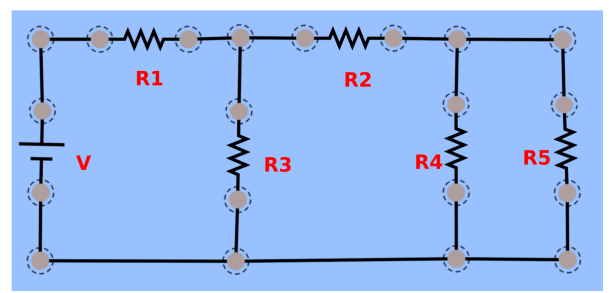
\includegraphics[scale=0.4]{../imgs/k0.png}
    \caption{circuito de práctica}
    \label{fig:1}
\end{figure}
Se armo el circuito de la figura \ref{fig:1} luego
medimos las resistencias con el multímetro, igual con las corrientes e igual con las caídas de potencial
con esto podemos sacar mallas y nodos para obtener una diferencia de volts.
\subsection*{Lista de Materiales}
A continuación se presenta una lista de materiales:
\begin{enumerate}
    \item Resistencias (varios)
    \item Multímetro (2)
    \item Cables banana(6)
    \item Protoboard
    \item Cables de conexión 
    \item Fuente de bajo voltaje 0-24 V
\end{enumerate}
\end{multicols}
\section{Resultados y análisis}\label{Resultados}			% -------------------- Resultados

\begin{table}[H]
\centering
\begin{tabular}{|c|c|c|}
    \hline
    n de resistencia & Resistencia k($\Omega$) & Unidad\\
    res 1 & 1.8 & kiloohms\\
    res 2 & 3.3 & kiloohms\\
    res 3 & 1.5 & kiloohms\\
    res 4 & 55 & kiloohms\\
    res 5 & 1 & kiloohms\\
    \hline
\end{tabular}
\caption{Resistencias individuales}
\label{tab:1}
\end{table}

\begin{table}[H]
\centering
\begin{tabular}{|c|c|c|}
    \hline
    & caídas de voltaje & Unidad\\
    res 1 & 2.6 & volts\\
    res 2 & 0.1862 & volts\\
    res 3 & 0.0521 & volts\\
    res 4 & 0.134 & volts\\
    res 5 & 0.1361 & volts\\
    \hline
\end{tabular}
\caption{Caídas de voltaje}
\label{tab:2}
\end{table}

\begin{table}[H]
\centering
\begin{tabular}{|c|c|c|}
    \hline
    R1 & 0.014 &Ampers\\
    R2 & 0.002 &Ampers\\
    R3 & 0.011 &Ampers\\
    R4 & 0.001 &Ampers\\
    R5 & 0.002 &Ampers\\
    \hline
\end{tabular}
\caption{Corriente}
\label{tab:3}
\end{table}

\begin{table}[H]
\centering
\begin{tabular}{|c|c|c|}
    \hline
    Malla 1 & Malla 2 & Malla 3\\
    \hline
    2.4138 & 0.3723	& 0.2701\\
    \hline
\end{tabular}
\caption{Mallas}
\label{tab:4}
\end{table}

Con respecto a la malla 1 de la tabla \ref{tab:4} la diferencia fue de 2.4 volts, idealmente el valor debería ser 0, las 
demás mallas tienen un valor cercano a 0.

\begin{table}[H]
\centering
\begin{tabular}{|c|c|}
    \hline
    Nodo 1 & Nodo 2\\ 
    \hline
    0.001 & 0.001 \\
    \hline
\end{tabular}
\caption{Nodos}
\label{tab:5}
\end{table}

Los nodos de la tabla \ref{tab:5} dan valores cercanos a 0.
\section{Conclusiones}\label{Conclusiones}				% -------------------- Conclusiones
Como equipo concluimos que el objetivo si cumplió en esta ocasión con básicamente casi cero error. 
También 
\begin{enumerate}
\item \textbf{Primera Ley o Ley de Nodos}: Establece que en cualquier nodo de un circuito eléctrico, la suma algebraica de las corrientes que entran y salen de dicho nodo es igual a cero. Esto se basa en el principio de conservación de la carga eléctrica.

\item \textbf{Segunda Ley o Ley de Mallas}: Enuncia que en cualquier lazo cerrado de un circuito eléctrico, la suma algebraica de las diferencias de potencial (tensiones) es igual a cerocite. Esto se deriva del principio de conservación de la energía.
\end{enumerate}
Estas leyes son esenciales para analizar y resolver circuitos eléctricos complejos, permitiendo determinar las corrientes y tensiones en cada componente del circuito
\begin{thebibliography}{9}						% -------------------- Bibliografía
	\bibitem{Latam}
    Latam, M. (2020). Leyes de Kirchhoff. Mecatrónica LATAM. https://www.mecatronicalatam.com/es/tutoriales/teoria/leyes-de-kirchhoff/
	\bibitem{Serway}
	Serway, R. A., $\&$ Jewett, J. W. (2008). Física para ciencias e ingeniería. (7.a
ed., Vol. 1). CENGAGE Learning.

\bibitem{Pérez}
	Newton, I. (1687). Philosophiæ Naturalis Principia Mathematica [Mathematical Principles of Natural Philosophy]. Londini: Jussu Societatis Regiæ ac Typis Josephi Streater.

\end{thebibliography}
\end{document}	